\documentclass[11pt,a4paper]{article}
\usepackage{fontspec,xeCJK}
\IfFontExistsTF{Microsoft JhengHei}{
  \setCJKmainfont{Microsoft JhengHei}
  \setCJKsansfont{Microsoft JhengHei}
  \setCJKmonofont{Microsoft JhengHei}
}{
  \setCJKmainfont{Noto Serif CJK TC}
  \setCJKsansfont{Noto Sans CJK TC}
  \setCJKmonofont{Noto Sans CJK TC}
}
\usepackage[margin=22mm,headheight=15pt]{geometry}
\usepackage{amsmath,amssymb,graphicx,booktabs,longtable,array,xcolor,hyperref,listings,fancyhdr}
\definecolor{accent}{HTML}{173C57}
\hypersetup{colorlinks=true,linkcolor=accent,urlcolor=accent,pdftitle={DIC06 - 等效閘極電容}}
\setlength{\parindent}{0pt}
\setlength{\parskip}{5pt}
\setlength{\emergencystretch}{3em}
\renewcommand{\arraystretch}{1.2}
\lstset{basicstyle=\ttfamily\small,breaklines=true,columns=fullflexible,frame=single}
\pagestyle{fancy}
\fancyhf{}
\fancyhead[L]{\small DIC06 / 本次模型}
\fancyhead[R]{\small 實驗報告}
\fancyfoot[C]{\thepage}
\title{\color{accent}DIC06\\[4pt]等效閘極電容}
\author{依講義規格重寫之實驗報告}
\date{17 October 2026}
\usepackage[american]{circuitikz}
\usetikzlibrary{arrows.meta,positioning,calc,shapes.geometric}
\begin{document}
\maketitle
\begin{center}\small\textbf{中文版}\\
HSPICE S-2021.09 \quad | \quad 模型庫另行提供
\end{center}
\section{目的}
依 Lab 6（PDF 24--25 頁）比較實際 MOS 輸入負載與固定電容等效，檢查講義四組 8/16/24/32 fF 近似在本次模型是否成立。

\section{Spec 對照}
\begin{longtable}{p{0.31\linewidth}p{0.29\linewidth}p{0.31\linewidth}}
\toprule
講義要求（PDF頁） & 實作 & 驗證與界線 \\\midrule
步驟 1：表 6.1 四個案例（24--25） & 01\_gate\_load：NL=1--4 & 四例全部模擬 \\
比較 MOS 與固定電容波形／延遲（25） & 每個 MLOAD 對應 8 fF & 差異已量化，未宣稱近似相等 \\
\bottomrule
\end{longtable}


\section{電路與設計推導}
兩條路徑的驅動反相器相同：$W_n=0.6\,\mu$m、$W_p=1.8\,\mu$m、$L=0.25\,\mu$m。MOS 負載各為兩倍寬度 $1.2/3.6\,\mu$m；NL 個負載並接在同一驅動輸出，使用 MOS multiplicity 表示相同並聯單元，其輸出仍可切換。原始 case a 使用單倍負載、case b 將負載串接，與講義不同；已改成正確的兩倍、並聯負載。

手算 $C_g\approx C_{ox}(W_n+W_p)L$，$C_{ox}=\epsilon_{ox}/t_{ox}$。講義 $t_{ox}=5.4$ nm 對應每負載約 7.87 fF，只屬原模型；本次加密模型沒有可查驗的 $t_{ox}$，不冒用該數字。講義 W/L 的文字標示顛倒，本文採 W 為寬、L 為長。

\section{模擬設定}
本次為使用另行提供模型的教學改寫，電源為 1.0 V、溫度為 $25\,^{\circ}\mathrm C$。保留講義指定的拓樸、負載及比較尺寸；原講義的 2.5 V 製程結果不是本次模型的驗收數值。1 V 僅是模擬條件，不能視為模型的安全額定。所有 MOS 的 Bulk 明確接至相應電源軌。

HSPICE S-2021.09 使用 RUNLVL=6；保存波形、列印資料及原生量測。圖表由本次數據重繪；CSV 保存於各 Lab 的 results。完成模擬表示求解成功，並不代表製程可靠度已驗證。加密模型仍有被抑制的警告；既有診斷未取得可判讀的進一步內容，因此不宣稱警告無害或全部模型限制已滿足。

輸入 0.1 ns 邊緣、5 ns 週期；暫態 10 ns，列印 1 ps。每條路徑量測輸出 10--90\% 邊緣及輸入輸出 50\% 傳播延遲。

\section{結果與規格檢查}
四例求解與量測皆成功。下表單位 ps，MOS/C 分別指實際負載／固定電容。
\begin{center}\small
\begin{tabular}{llllll}
\toprule
NL & $C$ (fF) & $t_{pHL,MOS}$ & $t_{pHL,C}$ & $t_{pLH,MOS}$ & $t_{pLH,C}$ \\
\midrule
1 & 8 & 76.80 & 63.82 & 139.95 & 88.76 \\
2 & 16 & 112.89 & 85.88 & 241.42 & 127.05 \\
3 & 24 & 148.64 & 107.34 & 339.83 & 164.48 \\
4 & 32 & 184.10 & 128.38 & 439.90 & 201.64 \\
\bottomrule
\end{tabular}
\end{center}

\begin{figure}[htbp]
\centering
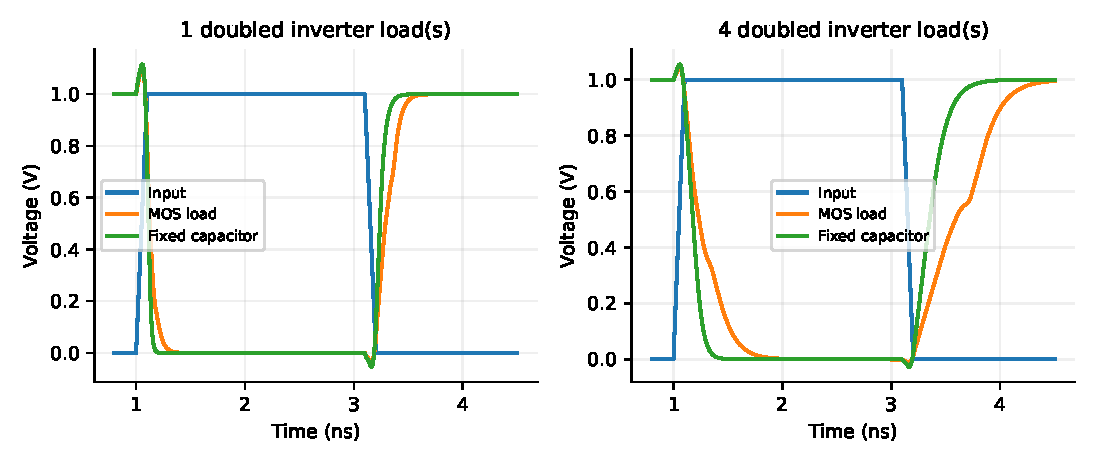
\includegraphics[width=\linewidth]{figures/gate_load_waveforms.pdf}
\caption{一個與四個負載的波形比較；由本次 HSPICE 數據重繪。}
\end{figure}

\begin{figure}[htbp]
\centering
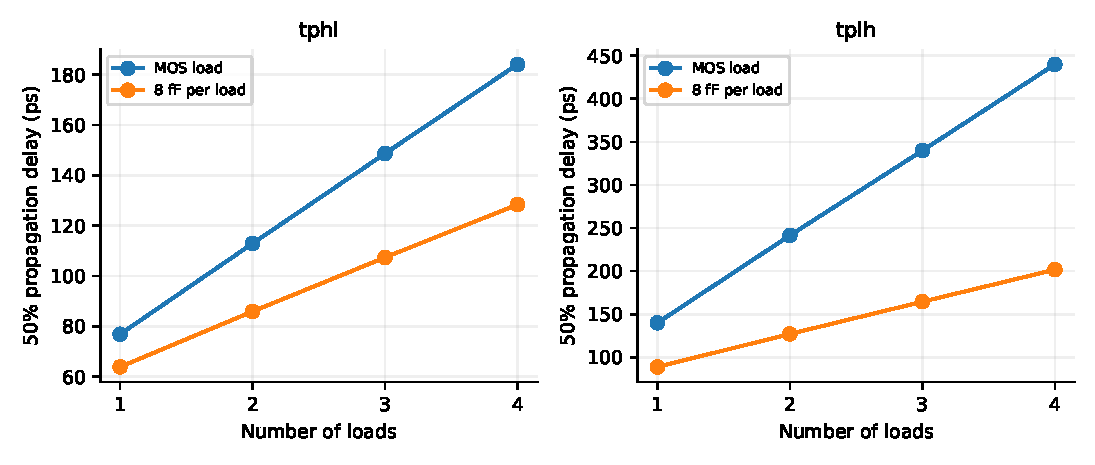
\includegraphics[width=\linewidth]{figures/gate_load_delays.pdf}
\caption{兩種負載的傳播延遲；由本次 HSPICE 數據重繪。}
\end{figure}


\section{討論}
MOS 負載在四個案例中皆比講義固定電容慢，尤其充電延遲：NL=4 為 439.90 ps，相較 32 fF 的 201.64 ps。差異來自本次模型的閘極電容、重疊／Miller 耦合及移動的負載輸出，不能只以單一 $C_{ox}WL$ 代表所有狀態。講義「近似相等」在本次條件下未重現，這是明確的模型移轉差異，不是省略實驗。

\section{結論}
四組要求已完整比較；8 fF/負載不是本次模型已驗證的等效值。若後續要建立標準元件庫，需另針對輸入 slew、輸出負載與邏輯狀態擬合有效電容。

\clearpage\section{MOS 電晶體電路圖}
來源：\texttt{01\_gate\_load.sp}。XDRV1 與 XDRV2 的 $W_n/W_p/L=0.6/1.8/0.25\,\mu$m。MOS 負載 MNLOAD／MPLOAD 的寬度加倍為 $1.2/3.6\,\mu$m，倍數 $M=N_L$，其中 $N_L=1,2,3,4$；汲極共接節點 z，與實際網表一致。

圖中沿用所列網表的元件與節點名稱；相同節點標籤表示電氣相連。除另有註明外，NMOS 的 bulk 接地，PMOS 的 bulk 接 $V_{DD}$。三端符號省略 bulk 導線以保持圖面清楚。
\begin{figure}[!htbp]\centering
\resizebox{12cm}{!}{\begin{circuitikz}[american,font=\small]

\begin{scope}[shift={(0,0)}]
\node[pmos] (D1p) at (0,1) {};
\node[nmos] (D1n) at (0,-1) {};
\draw (D1p.S) -- (0,2) node[above] {$V_{DD}$};
\draw (D1n.S) -- (0,-2) node[ground] {};
\draw (D1p.D) -- (0,0) -- (D1n.D);
\draw (D1p.G) -- (-1.15,1) -- (-1.15,-1) -- (D1n.G);
\draw (-1.15,0) node[circ] {} -- (-1.8,0) node[above] {in};
\draw (0,0) node[circ] {} -- (0.85,0) node[above] {ymos};
\node[right] at (0.25,1) {MP};
\node[right] at (0.25,-1) {MN};
\node at (0,2.6) {};
\coordinate (D1in) at (-1.8,0);
\coordinate (D1out) at (0.85,0);
\end{scope}

\begin{scope}[shift={(5,0)}]
\node[pmos] (Lp) at (0,1) {};
\node[nmos] (Ln) at (0,-1) {};
\draw (Lp.S) -- (0,2) node[above] {$V_{DD}$};
\draw (Ln.S) -- (0,-2) node[ground] {};
\draw (Lp.D) -- (0,0) -- (Ln.D);
\draw (Lp.G) -- (-1.15,1) -- (-1.15,-1) -- (Ln.G);
\draw (-1.15,0) node[circ] {} -- (-1.8,0) node[above] {ymos};
\draw (0,0) node[circ] {} -- (0.85,0) node[above] {z};
\node[right] at (0.25,1) {MP};
\node[right] at (0.25,-1) {MN};
\node at (0,2.6) {};
\coordinate (Lin) at (-1.8,0);
\coordinate (Lout) at (0.85,0);
\end{scope}
\draw (D1out) -- (Lin);
\end{circuitikz}}
\caption{MOS 負載支路：左側為 XDRV1，右側為倍數 $N_L$ 的 MNLOAD／MPLOAD；負載輸出 z 可隨輸入切換。}
\end{figure}
\begin{figure}[!htbp]\centering
\resizebox{6.7cm}{!}{\begin{circuitikz}[american,font=\small]

\begin{scope}[shift={(0,0)}]
\node[pmos] (D2p) at (0,1) {};
\node[nmos] (D2n) at (0,-1) {};
\draw (D2p.S) -- (0,2) node[above] {$V_{DD}$};
\draw (D2n.S) -- (0,-2) node[ground] {};
\draw (D2p.D) -- (0,0) -- (D2n.D);
\draw (D2p.G) -- (-1.15,1) -- (-1.15,-1) -- (D2n.G);
\draw (-1.15,0) node[circ] {} -- (-1.8,0) node[above] {in};
\draw (0,0) node[circ] {} -- (0.85,0) node[above] {ycap};
\node[right] at (0.25,1) {MP};
\node[right] at (0.25,-1) {MN};
\node at (0,2.6) {};
\coordinate (D2in) at (-1.8,0);
\coordinate (D2out) at (0.85,0);
\end{scope}
\draw (D2out) -- (2,0) to[C,l=$N_L\cdot8\,\mathrm{fF}$] (2,-2) node[ground] {};
\end{circuitikz}}
\caption{電容比較支路 XDRV2。兩個驅動器接收相同輸入波形。}
\end{figure}

\end{document}
